\documentclass[12pt,letterpaper]{article}\usepackage[]{graphicx}\usepackage[]{color}
%% maxwidth is the original width if it is less than linewidth
%% otherwise use linewidth (to make sure the graphics do not exceed the margin)
\makeatletter
\def\maxwidth{ %
  \ifdim\Gin@nat@width>\linewidth
    \linewidth
  \else
    \Gin@nat@width
  \fi
}
\makeatother

\definecolor{fgcolor}{rgb}{0.345, 0.345, 0.345}
\newcommand{\hlnum}[1]{\textcolor[rgb]{0.686,0.059,0.569}{#1}}%
\newcommand{\hlstr}[1]{\textcolor[rgb]{0.192,0.494,0.8}{#1}}%
\newcommand{\hlcom}[1]{\textcolor[rgb]{0.678,0.584,0.686}{\textit{#1}}}%
\newcommand{\hlopt}[1]{\textcolor[rgb]{0,0,0}{#1}}%
\newcommand{\hlstd}[1]{\textcolor[rgb]{0.345,0.345,0.345}{#1}}%
\newcommand{\hlkwa}[1]{\textcolor[rgb]{0.161,0.373,0.58}{\textbf{#1}}}%
\newcommand{\hlkwb}[1]{\textcolor[rgb]{0.69,0.353,0.396}{#1}}%
\newcommand{\hlkwc}[1]{\textcolor[rgb]{0.333,0.667,0.333}{#1}}%
\newcommand{\hlkwd}[1]{\textcolor[rgb]{0.737,0.353,0.396}{\textbf{#1}}}%

\usepackage{framed}
\makeatletter
\newenvironment{kframe}{%
 \def\at@end@of@kframe{}%
 \ifinner\ifhmode%
  \def\at@end@of@kframe{\end{minipage}}%
  \begin{minipage}{\columnwidth}%
 \fi\fi%
 \def\FrameCommand##1{\hskip\@totalleftmargin \hskip-\fboxsep
 \colorbox{shadecolor}{##1}\hskip-\fboxsep
     % There is no \\@totalrightmargin, so:
     \hskip-\linewidth \hskip-\@totalleftmargin \hskip\columnwidth}%
 \MakeFramed {\advance\hsize-\width
   \@totalleftmargin\z@ \linewidth\hsize
   \@setminipage}}%
 {\par\unskip\endMakeFramed%
 \at@end@of@kframe}
\makeatother

\definecolor{shadecolor}{rgb}{.97, .97, .97}
\definecolor{messagecolor}{rgb}{0, 0, 0}
\definecolor{warningcolor}{rgb}{1, 0, 1}
\definecolor{errorcolor}{rgb}{1, 0, 0}
\newenvironment{knitrout}{}{} % an empty environment to be redefined in TeX

\usepackage{alltt}
\usepackage[utf8]{inputenc}
\usepackage[margin=.7in]{geometry}
\usepackage{graphicx}
\usepackage{titling}
\usepackage{amsmath}
\usepackage{amsfonts}
\usepackage{amssymb}
\renewcommand{\theenumiv}{\arabic{enumiv}}
\setlength{\droptitle}{-5em}
\author{Maurice Diesendruck}
\title{MCMC Midterm 2: Attachments}
\IfFileExists{upquote.sty}{\usepackage{upquote}}{}
\begin{document}
\maketitle

% Question 5 Plots
\begin{center}
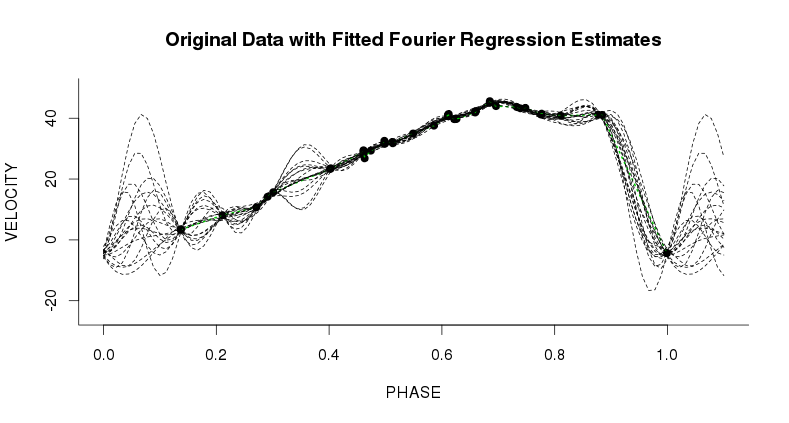
\includegraphics[height=8cm, keepaspectratio]{origdatawithfits.png}\\
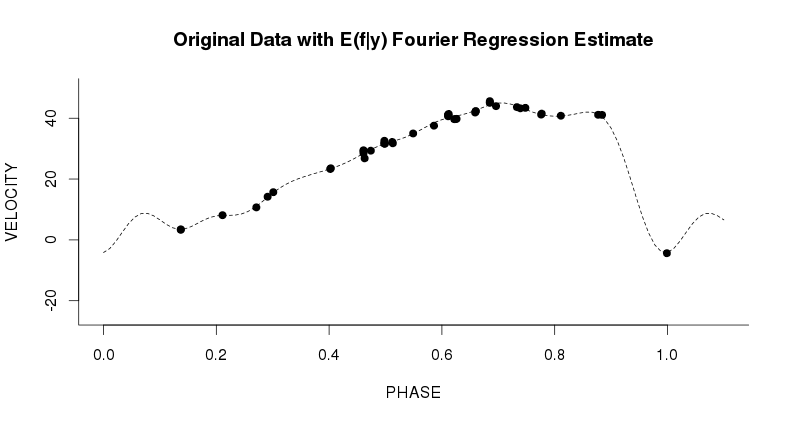
\includegraphics[height=8cm, keepaspectratio]{expected-f.png}\\
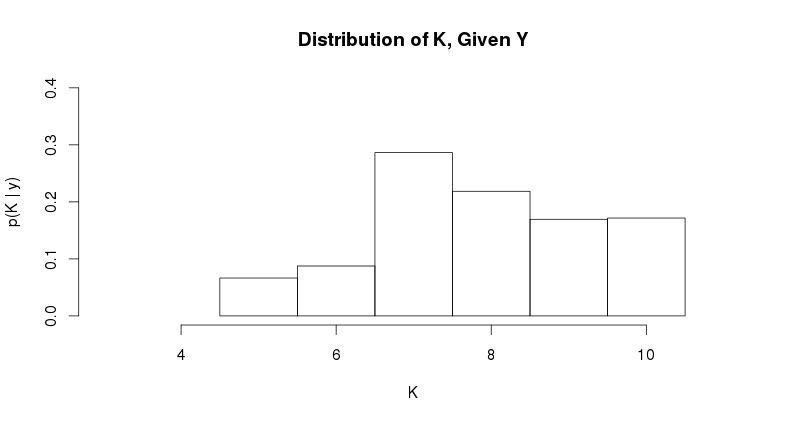
\includegraphics[height=8cm, keepaspectratio]{distribution-K.png}\\
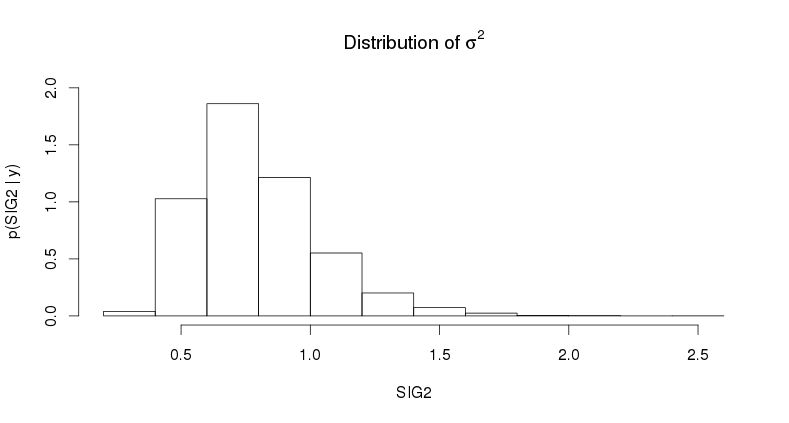
\includegraphics[height=8cm, keepaspectratio]{distribution-sig2.png}\\
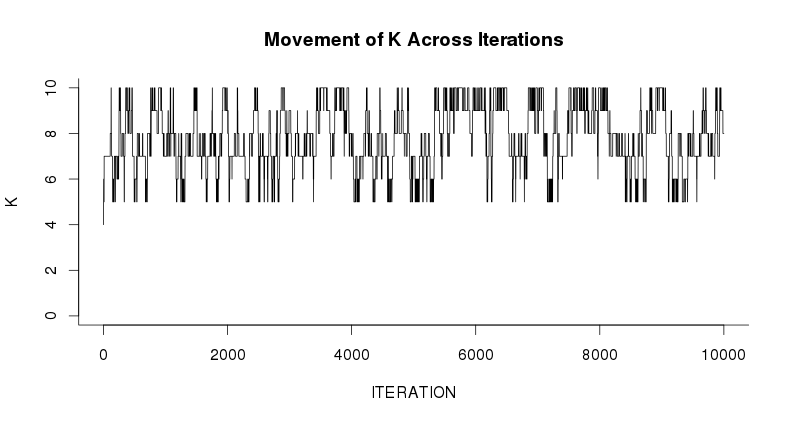
\includegraphics[height=8cm, keepaspectratio]{K-vs-iterations.png}\\
\end{center}

% Question 6 Plot
\begin{knitrout}
\definecolor{shadecolor}{rgb}{0.969, 0.969, 0.969}\color{fgcolor}
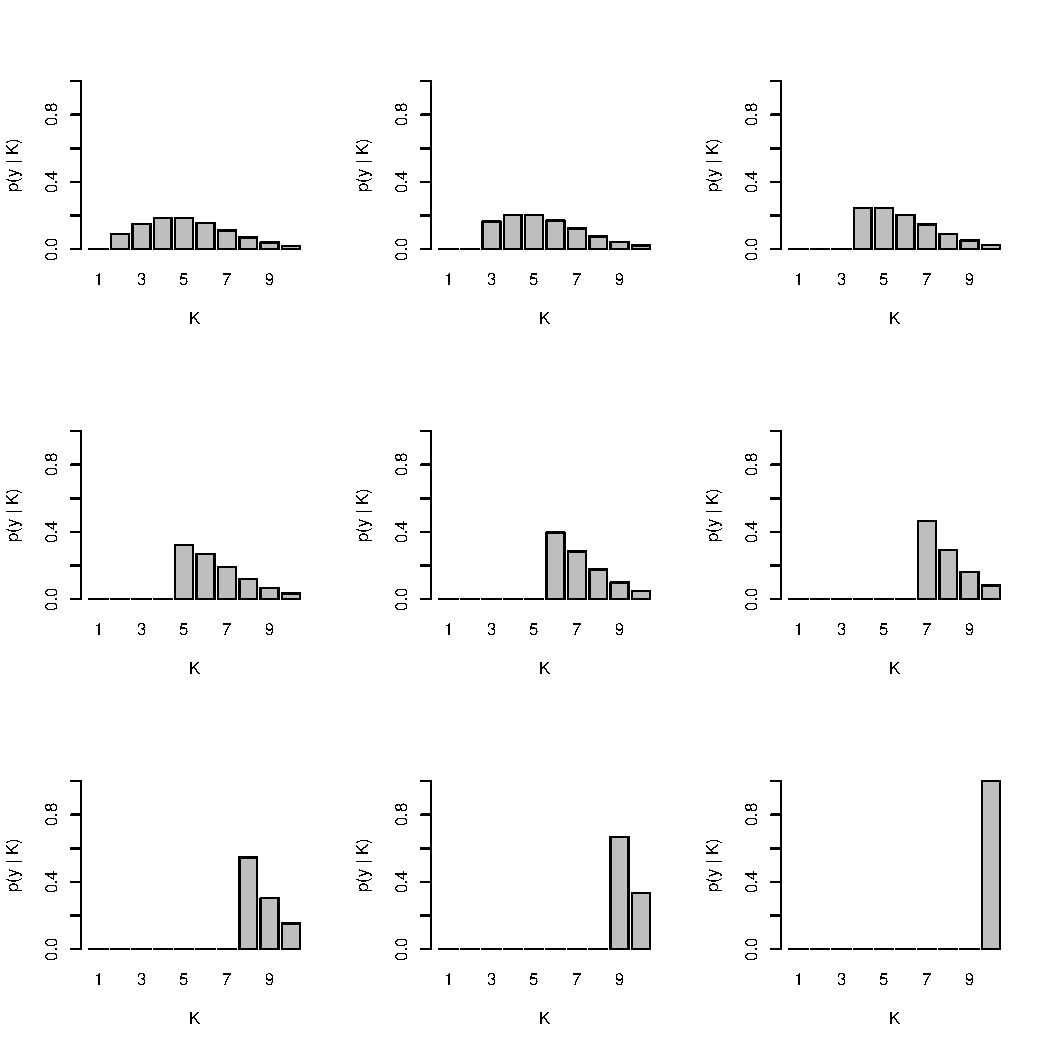
\includegraphics[width=\maxwidth]{figure/unnamed-chunk-1-1} 

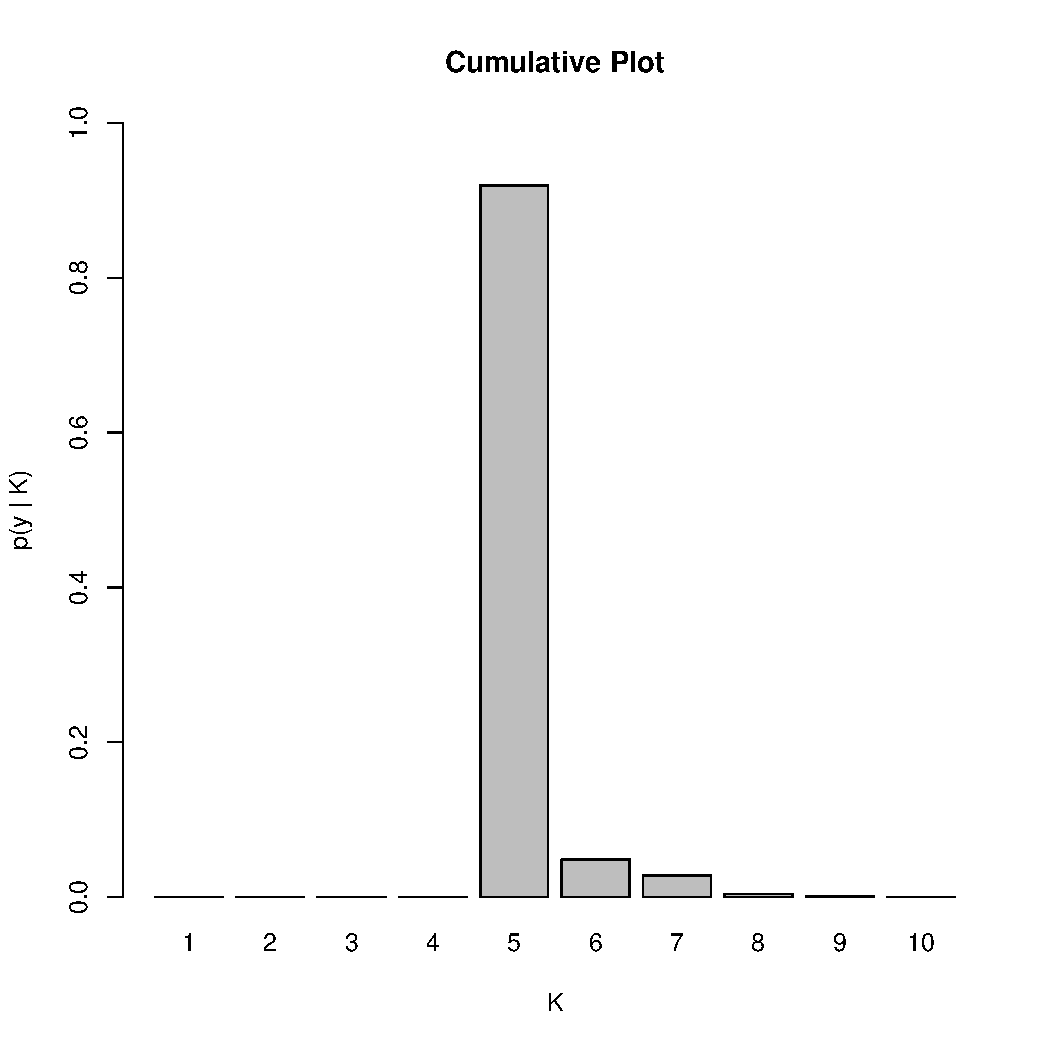
\includegraphics[width=\maxwidth]{figure/unnamed-chunk-1-2} 

\end{knitrout}

\section*{Relevant Code Snippets}

\subsection{Log Joint Posterior for Ratio}
\begin{knitrout}
\definecolor{shadecolor}{rgb}{0.969, 0.969, 0.969}\color{fgcolor}\begin{kframe}
\begin{alltt}
\hlstd{ljointpost}\hlkwb{=}\hlkwa{function}\hlstd{(}\hlkwc{K}\hlstd{,} \hlkwc{b}\hlstd{,} \hlkwc{sig2}\hlstd{)\{}
  \hlcom{#print("calculating posterior with param:");}
  \hlstd{n} \hlkwb{=} \hlkwd{length}\hlstd{(y);}
  \hlstd{p} \hlkwb{<-} \hlkwd{length}\hlstd{(b)}
  \hlstd{yhat} \hlkwb{<-} \hlstd{X[,}\hlnum{1}\hlopt{:}\hlstd{p]} \hlopt \hlstd{b}

  \hlcom{# Posterior. Cancel out terms without K, yhat, b.}
  \hlstd{lpo}  \hlkwb{<-} \hlstd{(}\hlopt{-}\hlnum{1}\hlopt{/}\hlnum{2}\hlstd{)}\hlopt{*}\hlstd{(}\hlnum{1}\hlopt{/}\hlstd{sig2)}\hlopt{*}\hlkwd{sum}\hlstd{((y}\hlopt{-}\hlstd{yhat)}\hlopt{^}\hlnum{2}\hlstd{)} \hlopt{-} \hlnum{1}\hlopt{/}\hlnum{2}\hlopt{*}\hlkwd{sum}\hlstd{(b}\hlopt{^}\hlnum{2}\hlstd{)}\hlopt{/}\hlnum{10} \hlopt{+} \hlstd{K}\hlopt{*}\hlkwd{log}\hlstd{(lambda)} \hlopt{-}
            \hlkwd{log}\hlstd{(}\hlkwd{factorial}\hlstd{(K))}

  \hlkwd{return}\hlstd{(lpo);}
\hlstd{\}}
\end{alltt}
\end{kframe}
\end{knitrout}

\subsection{Gibbs Conditional Posterior Distributions}
\begin{knitrout}
\definecolor{shadecolor}{rgb}{0.969, 0.969, 0.969}\color{fgcolor}\begin{kframe}
\begin{alltt}
\hlstd{sample.b} \hlkwb{<-} \hlkwa{function}\hlstd{(}\hlkwc{K}\hlstd{,}\hlkwc{sig2}\hlstd{) \{} \hlcom{# generate b ~ p(b | K, sig2, y)}
  \hlstd{idx} \hlkwb{<-} \hlnum{1}\hlopt{:}\hlstd{(}\hlnum{2}\hlopt{*}\hlstd{K}\hlopt{+}\hlnum{1}\hlstd{)}   \hlcom{# select columns (elements) for K harmonics}
  \hlstd{Xk} \hlkwb{<-} \hlstd{X[,idx]}      \hlcom{# Subset of design matrix, with 2K+1 columns.}
  \hlstd{A0k} \hlkwb{<-} \hlstd{A0[idx,idx]} \hlcom{# Precision matrix of beta prior.}
  \hlstd{b0k} \hlkwb{<-} \hlstd{b0[idx]}     \hlcom{# Mean vector of zeros from beta prior.}

  \hlcom{# Full conditionals from Question 2}
  \hlstd{V} \hlkwb{<-} \hlkwd{solve}\hlstd{(}\hlkwd{t}\hlstd{(Xk)}\hlopt\hlstd{Xk}\hlopt{/}\hlstd{sig2}\hlopt{+}\hlstd{A0k)}
  \hlstd{mm} \hlkwb{<-} \hlstd{V}\hlopt\hlstd{(}\hlkwd{t}\hlstd{(Xk)}\hlopt\hlstd{y}\hlopt{/}\hlstd{sig2)}
  \hlstd{L} \hlkwb{<-} \hlkwd{t}\hlstd{(} \hlkwd{chol}\hlstd{(V))}             \hlcom{# LL' = V}
  \hlstd{b} \hlkwb{<-} \hlstd{mm} \hlopt{+} \hlstd{L} \hlopt \hlkwd{rnorm}\hlstd{(}\hlnum{2}\hlopt{*}\hlstd{K}\hlopt{+}\hlnum{1}\hlstd{)} \hlcom{# b ~ N(m,V)}

  \hlkwd{return} \hlstd{(b)}
\hlstd{\}}

\hlstd{sample.sig2} \hlkwb{<-} \hlkwa{function}\hlstd{(}\hlkwc{K}\hlstd{,}\hlkwc{b}\hlstd{) \{} \hlcom{# generate 1/sig2 ~ p(1/sig2 | K,b,y)}
  \hlstd{p} \hlkwb{<-} \hlkwd{length}\hlstd{(b)}
  \hlstd{idx} \hlkwb{<-} \hlnum{1}\hlopt{:}\hlstd{(}\hlnum{2}\hlopt{*}\hlstd{K}\hlopt{+}\hlnum{1}\hlstd{)}   \hlcom{# select columns (elements) for K harmonics}
  \hlstd{Xk} \hlkwb{<-} \hlstd{X[,idx]}      \hlcom{# Subset of design matrix, with 2K+1.}

  \hlstd{a1} \hlkwb{<-} \hlstd{(n}\hlopt{/}\hlnum{2}\hlstd{)}\hlopt{+}\hlnum{1}
  \hlstd{b1} \hlkwb{<-} \hlkwd{t}\hlstd{(y}\hlopt{-}\hlstd{Xk}\hlopt\hlstd{b)}\hlopt\hlstd{(y}\hlopt{-}\hlstd{Xk}\hlopt\hlstd{b)}\hlopt{/}\hlnum{2} \hlopt{+} \hlnum{1}

  \hlstd{sig2inv} \hlkwb{<-} \hlkwd{rgamma}\hlstd{(}\hlnum{1}\hlstd{,}\hlkwc{shape}\hlstd{=a1,}\hlkwc{rate}\hlstd{=b1)}
  \hlstd{sig2} \hlkwb{<-} \hlnum{1}\hlopt{/}\hlstd{sig2inv}
  \hlkwd{return} \hlstd{(sig2)}
\hlstd{\}}
\end{alltt}
\end{kframe}
\end{knitrout}

\subsection{Auxiliary Variable Transformation and Reverse Transformation}
\begin{knitrout}
\definecolor{shadecolor}{rgb}{0.969, 0.969, 0.969}\color{fgcolor}\begin{kframe}
\begin{alltt}
\hlstd{qu} \hlkwb{<-} \hlkwa{function}\hlstd{(}\hlkwc{K}\hlstd{,} \hlkwc{b}\hlstd{,} \hlkwc{sig2}\hlstd{) \{}
  \hlcom{## find m,L for mapping T: (b,u) -> b1,  below}
  \hlcom{## bnew = m + L*u, }
  \hlcom{## Use a regression of residuals on (K+1)-st harmonic}
  \hlcom{##     to determine m and L}
  \hlstd{idx} \hlkwb{<-} \hlnum{1}\hlopt{:}\hlstd{(}\hlnum{2}\hlopt{*}\hlstd{K}\hlopt{+}\hlnum{1}\hlstd{)}   \hlcom{# select columns (elements) for K harmonics}
  \hlstd{Xk} \hlkwb{<-} \hlstd{X[,idx]}      \hlcom{# Subset of design matrix, with columns for setting of K.}
  \hlstd{eps} \hlkwb{<-} \hlstd{y}\hlopt{-}\hlstd{Xk}\hlopt\hlstd{b}

  \hlstd{regression} \hlkwb{<-} \hlkwd{lm}\hlstd{(eps} \hlopt{~} \hlkwd{sin}\hlstd{((K}\hlopt{+}\hlnum{1}\hlstd{)}\hlopt{*}\hlnum{2}\hlopt{*}\hlstd{pi}\hlopt{*}\hlstd{x)} \hlopt{+} \hlkwd{cos}\hlstd{((K}\hlopt{+}\hlnum{1}\hlstd{)}\hlopt{*}\hlnum{2}\hlopt{*}\hlstd{pi}\hlopt{*}\hlstd{x))}
  \hlstd{mk} \hlkwb{<-} \hlstd{regression}\hlopt{$}\hlstd{coefficients[}\hlnum{2}\hlopt{:}\hlnum{3}\hlstd{]}
  \hlstd{Vk} \hlkwb{<-} \hlkwd{vcov}\hlstd{(regression)[}\hlnum{2}\hlopt{:}\hlnum{3}\hlstd{,}\hlnum{2}\hlopt{:}\hlnum{3}\hlstd{]}
  \hlstd{Lk} \hlkwb{<-} \hlkwd{t}\hlstd{(}\hlkwd{chol}\hlstd{(Vk))}
  \hlkwd{return} \hlstd{(}\hlkwd{list}\hlstd{(}\hlkwc{m}\hlstd{=mk,} \hlkwc{V}\hlstd{=Vk,} \hlkwc{L}\hlstd{=Lk))}
\hlstd{\}}

\hlstd{Tinv} \hlkwb{<-} \hlkwa{function}\hlstd{(}\hlkwc{K1}\hlstd{,}\hlkwc{b1}\hlstd{,}\hlkwc{sig2}\hlstd{) \{}
  \hlcom{## proposed (shorter) par vector}
  \hlcom{## bnew = m + Lu or u = L^-1 (bnew-m)}
  \hlstd{K} \hlkwb{<-} \hlstd{K1}\hlopt{-}\hlnum{1}
  \hlstd{p} \hlkwb{<-} \hlnum{2}\hlopt{*}\hlstd{K}\hlopt{+}\hlnum{1}
  \hlstd{b} \hlkwb{<-} \hlstd{b1[}\hlnum{1}\hlopt{:}\hlstd{p]}
  \hlstd{bnew} \hlkwb{<-} \hlstd{b1[}\hlkwd{c}\hlstd{(p}\hlopt{+}\hlnum{1}\hlstd{,p}\hlopt{+}\hlnum{2}\hlstd{)]}

  \hlcom{## back out auxiliary u, and logJ}
  \hlstd{fit} \hlkwb{<-} \hlkwd{qu}\hlstd{(K, b, sig2)}
  \hlstd{u} \hlkwb{<-} \hlkwd{solve}\hlstd{(fit}\hlopt{$}\hlstd{L)}\hlopt\hlstd{(bnew}\hlopt{-}\hlstd{fit}\hlopt{$}\hlstd{m)}
  \hlstd{logJ} \hlkwb{<-} \hlkwd{sum}\hlstd{(}\hlkwd{log}\hlstd{(}\hlkwd{diag}\hlstd{(fit}\hlopt{$}\hlstd{L)))}

  \hlkwd{return} \hlstd{(}\hlkwd{list}\hlstd{(}\hlkwc{b}\hlstd{=b,} \hlkwc{u}\hlstd{=u,} \hlkwc{logJ}\hlstd{=logJ))}
\hlstd{\}}
\end{alltt}
\end{kframe}
\end{knitrout}

\subsection{Acceptance Probability for Birth Move}
\begin{knitrout}
\definecolor{shadecolor}{rgb}{0.969, 0.969, 0.969}\color{fgcolor}\begin{kframe}
\begin{alltt}
\hlstd{rho} \hlkwb{<-} \hlkwa{function}\hlstd{(}\hlkwc{K}\hlstd{,} \hlkwc{b1}\hlstd{,} \hlkwc{b}\hlstd{,} \hlkwc{u}\hlstd{,} \hlkwc{logJ}\hlstd{,} \hlkwc{sig2}\hlstd{) \{}
  \hlcom{##  acceptance ratio for birth move,}
  \hlcom{##  moving from b -> (b,u)}
  \hlcom{# current parameter: b}
  \hlcom{# proposal:          b1}
  \hlstd{K1} \hlkwb{<-} \hlstd{K}\hlopt{+}\hlnum{1}

  \hlstd{lqu} \hlkwb{<-} \hlkwd{sum}\hlstd{(}\hlkwd{dnorm}\hlstd{(u,} \hlkwc{m}\hlstd{=}\hlnum{0}\hlstd{,} \hlkwc{sd}\hlstd{=}\hlnum{1}\hlstd{,} \hlkwc{log}\hlstd{=}\hlnum{TRUE}\hlstd{))} \hlcom{# TODO: Shouldn't this be dnorm?}

  \hlstd{ljointpostratio} \hlkwb{<-} \hlkwd{ljointpost}\hlstd{(K1, b1, sig2)} \hlopt{-} \hlkwd{ljointpost}\hlstd{(K, b, sig2)}

  \hlcom{# Priors and likelihood}
  \hlstd{rho} \hlkwb{<-} \hlkwd{exp}\hlstd{(ljointpostratio)}

  \hlcom{# Transition probabilities}
  \hlkwa{if} \hlstd{(K}\hlopt{==}\hlnum{1}\hlstd{) \{}
    \hlstd{rho} \hlkwb{<-} \hlstd{rho}\hlopt{*}\hlnum{2}
  \hlstd{\}} \hlkwa{else if} \hlstd{(K}\hlopt{==}\hlstd{Kmx}\hlopt{-}\hlnum{1}\hlstd{) \{}
    \hlstd{rho} \hlkwb{<-} \hlstd{rho}\hlopt{/}\hlnum{2}
  \hlstd{\}} \hlkwa{else} \hlstd{\{}
    \hlcom{# Scaling rule smoothely penalizes larger values of K.}
    \hlstd{birth.weight} \hlkwb{<-} \hlkwd{qbeta}\hlstd{((Kmx}\hlopt{-}\hlstd{K}\hlopt{+}\hlnum{0.01}\hlstd{)}\hlopt{/}\hlstd{Kmx,} \hlnum{1}\hlstd{,} \hlnum{5}\hlstd{)}
    \hlstd{rho} \hlkwb{<-} \hlstd{rho}\hlopt{*}\hlstd{birth.weight}
  \hlstd{\}}
  \hlstd{rho} \hlkwb{<-} \hlstd{rho}\hlopt{/}\hlkwd{exp}\hlstd{(lqu)}         \hlcom{# Auxiliary}
  \hlstd{rho} \hlkwb{<-} \hlstd{rho}\hlopt{*}\hlkwd{exp}\hlstd{(logJ)}        \hlcom{# Jacobian}

  \hlkwd{return} \hlstd{(rho)}
\hlstd{\}}
\end{alltt}
\end{kframe}
\end{knitrout}


\end{document}






